\section{Additional Experiments Results}
\label{section:Results:AdditionalExperimentResults}

\import{./tables/results/dataset_variance}{Average-metric-dataset-variance.tex}
\import{./tables/results/ttest}{ttest-p-values-variance-experiments-sMAPE.tex}
\import{./tables/results/ttest}{ttest-p-values-variance-experiments-MASE.tex}
The results of our two additional experiments are shown in \Cref{table:Average-metric-dataset-variance}.
The table shows the average metrics for all the time series in the dataset described in the name.
For example: \textit{dataset-high-variance-lstm-local-univariate} row show the average
results for the local univariate LSTM on the high variance dataset.

\subsection{CNN-AE-LSTM on variance}
The CNN-AE-LSTM got MASE of $0.645$ and an sMAPE of $0.864$
on the high variance dataset. The CNN-AE-LSTM (\textit{dataset-high-variance-cnn-ae-lstm-local-unviariate}) outperforms the LSTM on
the same dataset with an sMAPE of $0.832$ and a mase of $0.634$, which is an sMAPE reduction of $3.7\%$
and a relativily low p-value of $0.147$.

The CNN-AE-LSTM performs much worse than the LSTM on the low variance dataset,
whit a sMAPE of $0.641$ versus $0.421$, and a MASE of $5.072$ versus $3.740$.
This is a $33.3\%$ decreased sMAPE perfomance and a low p-value of $0.01$.
The MASE score is $26.3\%$ worse with a p-value of $0.053$.

On the medium variance dataset the CNN-AE-LSTM performs marginally better than the LSTM
with a sMAPE of $0.501$ versus $0.502$. Both models score the same MASE of $0.788$, the
p-value of $0.732$ is too high to say anything of value.


% \import{./tables/results/dataset_high_variance}{Average-metric-dataset-high-variance.tex}
% \import{./tables/results/ttest}{ttest-p_values-variance.tex}

\begin{figure}[h!]
  \centering
  \caption{Boxplot of predictions made on the high variance, and the low variance dataset, comparing CNN-AE-LSTM against LSTM}
  \begin{subfigure}[t]{0.49\textwidth}
    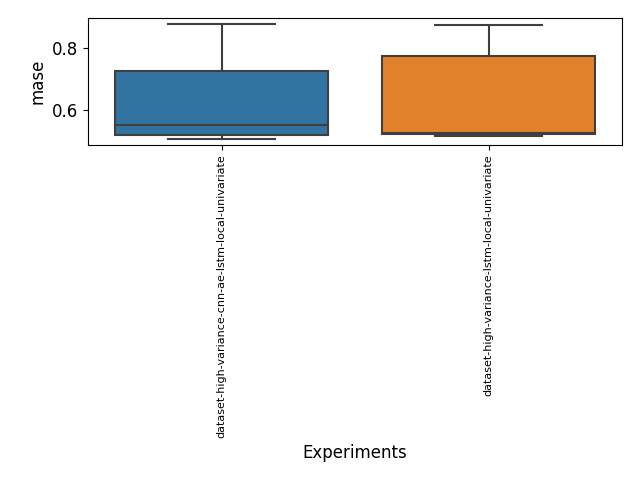
\includegraphics[width=\textwidth]{./figs/results/boxplot/mase-dataset_high_variance.png}
    \hfill
    \caption{MASE metrics from the high variance dataset.
      The CNN-AE-LSTM show improvements.
    }
    \label{fig:results:boxplot-mase-dataset-high-variance}

  \end{subfigure}
  \begin{subfigure}[t]{0.49\textwidth}
    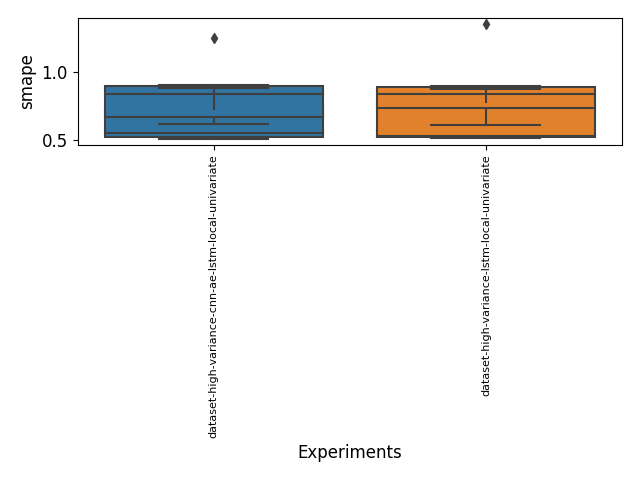
\includegraphics[width=\textwidth]{./figs/results/boxplot/smape-dataset_high_variance.png}
    \hfill
    \caption{sMAPE metrics from the high variance dataset.
      The CNN-AE-LSTM show
    }
    \label{fig:results:boxplot-smape-dataset-high-variance}
  \end{subfigure}
  \begin{subfigure}[b]{0.49\textwidth}
    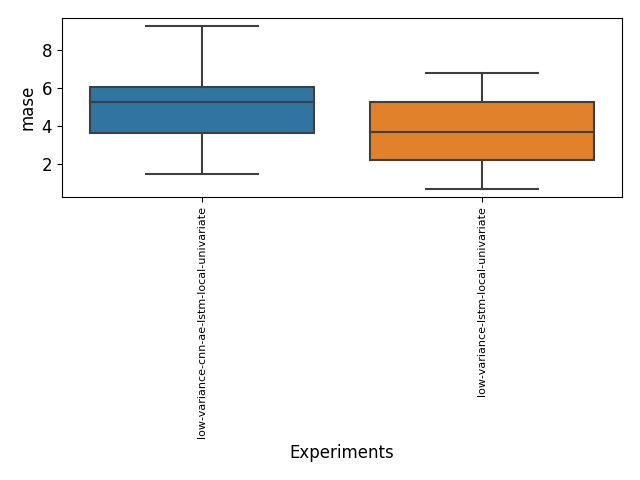
\includegraphics[width=\textwidth]{./figs/results/boxplot/mase-dataset_low_variance.png}
    \hfill
    \caption{MASE metrics from the low variance dataset}

  \end{subfigure}
  \begin{subfigure}[b]{0.49\textwidth}
    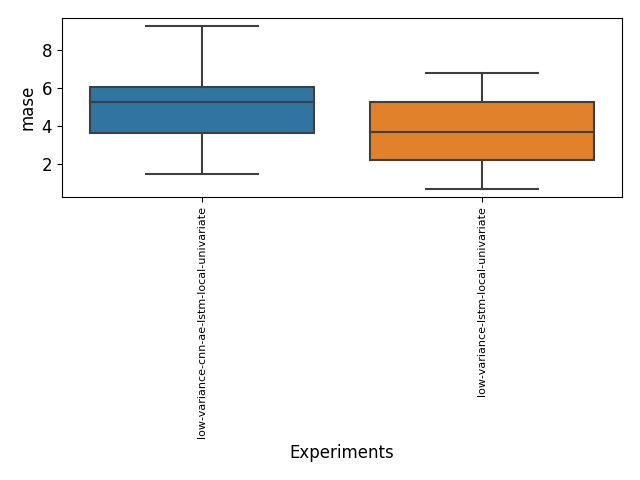
\includegraphics[width=\textwidth]{./figs/results/boxplot/mase-dataset_low_variance.png}
    \hfill
    \caption{sMAPE metrics from low variance dataset}

  \end{subfigure}
\end{figure}

\subsection{Differencing}
\import{./tables/results/dataset_diff}{Average-metric-dataset-diff.tex}
\import{./tables/results/ttest}{ttest-p-values-differencing-experiments-MASE.tex}




% \import{./tables/results/dataset_low_variance}{Average-metric-dataset-low-variance.tex}
% \import{./tables/results/dataset_seasonal_diff}{seasonal-local-univariate-lstm-differencing-dataset-seasonal-diff.tex}

% \import{./tables/results/dataset_diff}{seasonal-local-univariate-lstm-differencing-dataset-diff.tex}
% \import{./tables/results/dataset_diff}{local-univariate-lstm-dataset-1-dataset-diff.tex}
% \import{./tables/results/dataset_diff}{local-univariate-lstm-dataset-1-diff-dataset-diff.tex}

Comparing the local univariate LSTM with differencing done as a pre-processing step
on dataset 3 in \Cref{table:Average-metric-dataset-diff},
with the same model type, without differencing,
the original local univariate LSTM model without differencing scored a MASE of
$2.207$, a sMAPE of $0.488$, and a 7-day MASE of $1.345$.
The model with differencing scored a MASE of $1.866$, a sMAPE of $0.367$ and a 7-day MASE of
$0.916$. That is an improvement of $15.45\%$, $24.80\%$, and $31.90\%$ respectively; however, none of these improvements are not of statistical significans as the sMAPE p-value is as high as $0.503$.

We can, however, with greater confidence confirm that differencing on dataset 1 will decrease
the results by $15.38\%$, with a p-value of $0.183$.